Dans ce chapitre, nous étudions les outils et travaux existants pour l'édition collaborative de documents structurés, le chiffrement bout à bout et le stockage distribué.

\section{Définitions}
\subsection{Document structuré}
Un document structuré organise l'information de manière hiérarchique avec des éléments et attributs spécifiques. Il facilite la compréhension, la manipulation et la réutilisation des informations, contrairement aux documents non structurés.

Dans un tableau blanc collaboratif, un document structuré représente les éléments graphiques et textuels. Il aide à manipuler et modifier les éléments individuels, gérer l'historique des modifications et synchroniser les données entre les participants.

Le format SVG qui utilise le langage XML est un exemple de document structuré. Il est utilisé pour décrire la structure et le contenu d'un document vectoriel. Il est composé d'éléments graphiques, tels que des rectangles, des cercles et des lignes, et de textes.

\begin{listing}[H]
    \inputminted{XML}{assets/figure/svg-example.svg}
    \caption{Exemple de document SVG \label{fig:svg-example}}
\end{listing}

\subsection{Édition collaborative de documents}
L'édition collaborative permet à plusieurs utilisateurs de travailler simultanément sur un document en fusionnant les modifications en temps réel.
Plusieurs outils existent pour l'édition collaborative de documents structurés, un exemple connu est Google Docs.

\section{Méthodes et protocoles pour resoudre les conflits de modification}
Lors de l'édition collaborative de documents structurés, les utilisateurs peuvent modifier le document en même temps. Les modifications peuvent être effectuées sur des éléments différents ou sur le même élément. Dans ce cas, il y a un conflit de modification. Les conflits de modification peuvent être résolus de différentes manières, par exemple en utilisant un mécanisme de verrouillage ou en utilisant un algorithme de fusion. Dans cette section, nous aborderons les méthodes et protocoles pour résoudre les conflits de modification.

\subsection{Operational Transformation (OT)}
La Transformation Opérationnelle (OT) est un mécanisme de synchronisation de données en temps réel qui résout les conflits entre modifications concurrentes apportées par les utilisateurs. L'OT repose sur la transformation des opérations pour préserver leur intention lorsqu'elles sont appliquées dans un ordre différent. Dans cette section, nous aborderons les concepts clés, les mécanismes et les systèmes basés sur l'OT.

\subsubsection{Concepts de base}
Pour comprendre le fonctionnement de l'OT, il est important de se familiariser avec les concepts de base suivants:

\paragraph{Opération:} Une opération est une action effectuée par un utilisateur sur un document, telle que l'insertion ou la suppression d'un caractère. Les opérations sont généralement représentées par des objets contenant des informations sur l'action effectuée, la position dans le document et, le cas échéant, le caractère inséré ou supprimé.
\paragraph{Intention:} L'intention d'une opération est l'effet souhaité de l'opération sur le document. L'OT vise à préserver l'intention des opérations, même lorsqu'elles sont appliquées dans un ordre différent.
\paragraph{Conflit:} Un conflit se produit lorsque deux opérations sont effectuées simultanément sur le même document, et que l'application de ces opérations dans un ordre différent peut entraîner des résultats incohérents. L'OT résout les conflits en transformant les opérations concurrentes de manière à préserver leur intention.

\subsubsection{Transformation des opérations}
La transformation des opérations (OT) permet de préserver l'intention des opérations concurrentes en les modifiant. Prenons Alice et Bob travaillant sur un document, leurs opérations étant $O_A$ et $O_B$. L'OT utilise les fonctions de transformation $T_1$ et $T_2$ pour résoudre les conflits :

\begin{equation}
    \begin{aligned}
        O_A' = T_1(O_A, O_B) \\
        O_B' = T_2(O_B, O_A)
    \end{aligned}
\end{equation}

Les opérations transformées $O_A'$ et $O_B'$, appliquées au document, préservent l'intention et résolvent les conflits.

\subsubsection{Conditions de transformation}
La transformation opérationnelle (OT) est un algorithme essentiel pour assurer la cohérence des documents lors de modifications simultanées par plusieurs utilisateurs. Les conditions de transformation, appelées propriétés de transformation (TP), sont définies pour préserver les intentions des utilisateurs et obtenir un document final cohérent.

Une propriété peut garantir que les opérations transformées sont cohérentes, peu importe l'ordre d'application. D'autres conditions peuvent être ajoutées pour assurer l'équilibre et la cohérence des opérations transformées, comme celle-ci :

\begin{equation}
    \begin{aligned}
        T_1(O_A', O_B') = O_A \\
        T_2(O_B', O_A') = O_B
    \end{aligned}
\end{equation}

Cette formule exprime que les opérations initiales $O_A$ et $O_B$ sont retrouvées en transformant à nouveau les opérations transformées $O_A'$ et $O_B'$ l'une par rapport à l'autre.

En définissant des conditions de transformation appropriées, l'algorithme OT préserve les intentions des utilisateurs et garantit un document final cohérent, même en cas de travail simultané sur un même document.
\subsubsection{Algorithmes OT}
Plusieurs algorithmes et systèmes OT ont émergé au fil du temps. En voici quelques exemples notables:

\subsubsection{Algorithme Jupiter}
Jupiter, un système de collaboration en temps réel OT, fut créé au début des années 1990 au Xerox PARC pour répondre à la demande croissante de collaboration en ligne sur des documents partagés. Clarence Ellis dirigea ce projet, qui aboutit à la publication d'un article\cite{sunOperationalTransformationRealTime1998} en 1998 présentant les concepts clés et les algorithmes OT. Ellis avait déjà publié un article\cite{ellisConcurrencyControlGroupware1989} en 1989, posant les bases pour le développement de Jupiter.

Jupiter fonctionne en client-serveur, chaque client et serveur possédant sa propre copie du document et appliquant les opérations localement. Les opérations sont transmises au serveur, transformées, puis redistribuées. Jupiter utilise un mécanisme de contrôle de causalité pour garantir un ordre préservant les relations causales.

Malgré l'absence de développement actif, Jupiter influence toujours de nombreux systèmes de collaboration en temps réel.

\subsubsection{Algorithme Google Wave}
Google Wave\cite{incIntroducingGoogleWave2009}, annoncé en 2009, était un système de collaboration en temps réel conçu par Google. Combinant messagerie instantanée, courrier électronique, partage de documents et médias sociaux, il visait à faciliter la communication et la collaboration en ligne.

Basé sur l'OT, Google Wave utilisait un modèle décentralisé où chaque utilisateur maintenait sa propre copie du document. Cela offrait plus de flexibilité pour gérer les modifications hors ligne et synchroniser les données lorsqu'un utilisateur se reconnectait.

Cependant, Google Wave ne parvint pas à attirer suffisamment d'utilisateurs et son développement fut arrêté en 2010\cite{holzleOfficialGoogleBlog2010}. Néanmoins, certaines idées et techniques furent intégrées dans d'autres produits de collaboration en temps réel de Google, tels que Google Docs, et des projets open source comme Apache Wave\cite{foundationApacheWave2012} et ShareDB\cite{smithShareDBRealtimeDocument2014}.

\subsubsection{Limitations et défis de l'OT}
Bien que l'OT soit un mécanisme puissant pour la synchronisation en temps réel des documents et la résolution des conflits, il présente également certaines limitations et défis:

\paragraph{Complexité:} Les algorithmes basés sur l'OT peuvent être complexes à mettre en oeuvre et à déboguer, en particulier lorsqu'ils doivent gérer des cas de conflits complexes et des relations de causalité.
\paragraph{Performances:} La transformation des opérations et le contrôle de la causalité peuvent avoir un impact sur les performances, surtout lorsque le nombre d'utilisateurs et d'opérations concurrentes augmente.
\paragraph{Interopérabilité:} Les systèmes basés sur l'OT peuvent avoir des difficultés à interagir avec d'autres systèmes de synchronisation de données qui n'utilisent pas l'OT, ce qui peut limiter leur applicabilité dans certaines situations.
\paragraph{Sémantique des opérations:} Les fonctions de transformation doivent être définies pour chaque type d'opération et chaque structure de données, ce qui peut être délicat lorsque les opérations ont des sémantiques complexes ou interdépendantes.

Malgré ces défis, l'OT reste une méthode importante et largement utilisée pour la collaboration en temps réel et la synchronisation des données dans les systèmes distribués.

\subsection{Conflict-Free Replicated Data Types (CRDT)}
Les CRDT (Conflict-Free Replicated Data Types) sont conçus pour résoudre les conflits de manière déterministe lors de la collaboration en temps réel sur des documents partagés, sans serveur central. Ils sont commutatifs et idempotents, garantissant ainsi la cohérence et la convergence des documents dans un environnement distribué et répliqué.

\subsubsection{Fonctionnement des CRDT}
Les CRDT sont distribués et répliqués sur plusieurs machines, chaque client ayant sa propre copie des données. Les clients peuvent modifier les données et les synchroniser entre eux, avec des identifiants uniques pour garantir la commutativité et l'idempotence des opérations.

\subsubsection{Exemple d'utilisation de CRDT}
Considérons un exemple simple pour illustrer l'utilisation des CRDT et mettre en évidence les différences avec l'OT. Supposons que deux utilisateurs, Alice et Bob, collaborent sur un document texte initialisé avec le mot "chat".

Dans l'algorithme Logoot, chaque position de caractère est associée à un identifiant unique. Les identifiants sont des listes d'entiers de taille variable, appelées positions. Les positions sont comparées lexicographiquement pour déterminer l'ordre des caractères dans le document.

\paragraph{Scénario}
Alice et Bob travaillent sur un texte initial "chat". Alice veut former "chou" en ajoutant "ou" après "ch", pendant que Bob veut former "chef" en ajoutant "ef" après "ch".

\paragraph{Logoot CRDT}
Voici comment Alice et Bob peuvent collaborer sur le document texte en utilisant Logoot CRDT en se concentrant seulement sur l'étape d'insertion:

\begin{equation}
    c(1),\ h(2), \ a(3), t(4) \quad \text{(chat)}
\end{equation}

Alice insère "ou" après "ch" et génère de nouvelles positions :

\begin{equation}
    o(2, 1), \ u(2, 2)
\end{equation}

Le texte d'Alice devient :

\begin{equation}
    c(1), \ h(2), \ o(2, 1), \ u(2, 2), \ a(3), \ t(4) \quad \text{(chouat)}
\end{equation}

Bob insère "ef" après "ch" et génère aussi de nouvelles positions :

\begin{equation}
    e(2, 3), f(2, 4)
\end{equation}

Le texte de Bob devient :

\begin{equation}
    c(1), \ h(2), \ e(2, 3), \ f(2, 4), \ a(3), \ t(4) \quad \text{(chefat)}
\end{equation}

Les opérations d'insertion sont échangées.

Alice intègre l'insertion de Bob :

\begin{equation}
    c(1), \ h(2), \ o(2, 1), \ u(2, 2), \ e(2, 3), \ f(2, 4), \ a(3), \ t(4) \quad \text{(chouefat)}
\end{equation}

Bob intègre l'insertion d'Alice :

\begin{equation}
    c(1), \ h(2), \ o(2, 1), \ u(2, 2), \ e(2, 3), \ f(2, 4), \ a(3), \ t(4) \quad \text{(chouefat)}
\end{equation}

Le résultat est identique pour Alice et Bob, malgré un ordre différent d'opérations. Les CRDT assurent convergence et cohérence sans transformation opérationnelle.
\subsubsection{CRDT dans les algorithmes et systèmes}
Les CRDT inspirent de nombreux algorithmes et systèmes de collaboration en temps réel, tels que WOOT, Treedoc, RGA, Logoot, LSEQ, Automerge, Yjs et Riak.

\paragraph{Automerge\cite{hardenbergAutomerge2023}: } Automerge est une bibliothèque JavaScript pour développer des applications collaboratives en temps réel, comme des éditeurs de texte et des tableaux Kanban. Elle utilise des CRDT pour synchroniser les données entre les instances de l'application, en maintenant la cohérence et en résolvant les conflits.

\paragraph{Yjs\cite{nicolaescuYjsFrameworkRealTime2015}: } Yjs est une bibliothèque JavaScript de collaboration en temps réel qui utilise aussi les CRDT pour la synchronisation des données. Yjs supporte diverses structures de données et fonctionnalités, dont la collaboration sur des documents texte, des tableaux et des graphes.

\paragraph{Riak\cite{amazon.comRiakDynamoAmazon2007}: } Riak est une base de données distribuée et décentralisée conçue pour offrir une grande disponibilité et une tolérance aux partitions. Riak utilise des CRDT pour assurer la cohérence des données entre les n\oe udss du système, permettant aux clients d'effectuer des opérations de lecture et d'écriture même en cas de défaillance partielle du réseau.

En bref, les CRDT sont une approche intéressante pour la collaboration en temps réel. Elles résolvent les problèmes de synchronisation et de cohérence des données sans recourir à la transformation opérationnelle. Toutefois, les CRDT ne conviennent pas à tous les types de données et structures de données, et leur mise en œuvre peut être complexe.

\section{Zéro Trust}
Le modèle Zéro Trust est une approche de cybersécurité basée sur l'idée de ne faire confiance à aucune entité, interne ou externe, dans un système informatique. On vérifie constamment les identités et les autorisations avant d'accorder l'accès aux ressources. Cette méthode réduit les risques de failles de sécurité et protège les données sensibles contre les accès non autorisés.

\section{Chiffrement bout à bout}
Le chiffrement bout à bout (E2EE) est un système de communication qui garantit que seuls les utilisateurs participant à la conversation peuvent lire les messages échangés. Il vise à protéger la confidentialité des communications en empêchant les tiers, tels que les fournisseurs de télécommunications, les acteurs malveillants et même les fournisseurs de services, d'accéder aux clés de chiffrement nécessaires pour déchiffrer les messages. Ainsi, seul l'expéditeur et les destinataires légitimes peuvent lire ou modifier les données échangées. L'expéditeur chiffre les messages, et le tiers ne dispose pas des moyens pour les déchiffrer, les stockant donc sous forme chiffrée. Les destinataires récupèrent les données chiffrées et les déchiffrent eux-mêmes, assurant ainsi la confidentialité de la communication.
\subsection{Fonctionnement du chiffrement bout à bout}
Le chiffrement bout à bout utilise des clés de chiffrement asymétriques pour chaque utilisateur participant à une communication sécurisée. Chaque utilisateur possède une paire de clés, une publique et une privée. La clé publique est partagée librement, tandis que la clé privée reste secrète et accessible uniquement à l'utilisateur concerné.

Pour envoyer un message chiffré, un utilisateur A utilise la clé publique de l'utilisateur B pour chiffrer le message. Une fois chiffré, seul B peut déchiffrer le message avec sa clé privée. Ce processus est également appelé chiffrement asymétrique.

Par exemple, dans une application de messagerie chiffrée bout à bout, Alice utilise la clé publique de Bob pour chiffrer un message. Le message chiffré est envoyé et stocké sur le serveur de messagerie. Même si le serveur est compromis ou que les données sont interceptées, le message reste illisible sans la clé privée de Bob. Bob déchiffre ensuite le message avec sa clé privée.

Le partage des clés de chiffrement doit être effectué avec prudence pour éviter leur interception. Les clés doivent être échangées de manière sécurisée, en utilisant un canal de communication sûr.

\section{Bases de données immuables}
Les bases de données immuables, comme Immudb\cite{incImmuDB2023}, préservent l'intégrité et l'auditabilité des données en empêchant leur modification ou suppression une fois ajoutées. Les nouvelles données sont ajoutées sous forme d'événements ou de transactions, et les anciennes restent inchangées, créant un historique complet et vérifiable des modifications. Une des structures de données utilisées pour assurer l'intégrité et l'authenticité des données dans ce type de base de données est l'arbre de Merkle (voir la figure \ref{merkle}).

\begin{figure}[!htb]
    \begin{center}
        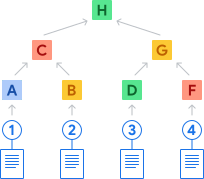
\includegraphics[]{\assetsdir/merkle-tree.svg}
    \end{center}
    \caption[Arbre de Merkle]{\label{merkle} L'arbre de Merkle illustre la structure de données utilisée pour vérifier l'intégrité et l'authenticité des données dans une base de données immuable. Les feuilles de l'arbre représentent les empreintes cryptographiques des données, tandis que les n\oe uds internes sont les empreintes cryptographiques des n\oe uds enfants. Cette structure permet de créer un registre vérifiable qui préserve l'historique des enregistrements et garantit l'inaltérabilité des données.}
\end{figure}

\section{Conclusion}
En conclusion, l'état de l'art dans le domaine de l'édition collaborative de documents, du chiffrement bout à bout et du stockage distribué montre qu'il existe plusieurs approches pour aborder ces problématiques. Les systèmes basés sur resolution de conflits, tels que Jupiter et Google Wave, ont apporté des contributions significatives dans la synchronisation des données en temps réel et la résolution des conflits. Cependant, des défis subsistent, tels que la complexité et les performances des algorithmes.

Face à ces défis, les chercheurs et les développeurs continuent d'explorer de nouvelles approches et d'améliorer les technologies existantes pour répondre aux besoins croissants en matière de collaboration, de sécurité et de décentralisation des données.